%%%  Ukázkový text a dokumentace stylu pro text závěrečné (bakalářské a
%%%  diplomové) práce na KI PřF UP v Olomouci
%%%  Copyright (C) 2012 Martin Rotter, <rotter.martinos@gmail.com>
%%%  Copyright (C) 2014 Jan Outrata, <jan.outrata@upol.cz>


%%  Pro získání PDF souboru dokumentu je třeba tento zdrojový text v
%%  LaTeXu přeložit (dvakrát) programem pdfLaTeX.

%%  V případě použití programu BibLaTeX pro tvorbu seznamu literatury
%%  je poté ještě třeba spustit program Biber s parametrem jméno
%%  souboru zdrojového textu bez přípony a následně opět (dvakrát)
%%  přeložit zdrojový text programem pdfLaTeX.

%%  Postup získání Postscriptového souboru je popsán v dokumentaci.


%%  Třída dokumentu implementující styl pro závěrečnou práci. Vybrané
%%  nepovinné parametry (ostatní v dokumentaci):

%%  'master' pro sazbu diplomové práce, jinak se sází bakalářská práce

%%  'field=kód' pro Váš studijní obor, kódy pro diplomovou práci 'uvt'
%%  pro Učitelství výpočetní techniky pro střední školy a 'binf' pro
%%  Bioinformatiku, jinak je výchozí Informatika, a pro bakalářskou
%%  práci 'ainfk' pro Aplikovanou informatiku v kombinované formě,
%%  'inf' pro Informatiku, 'infv' pro Informatiku pro vzdělávání a
%%  'binf' pro Bioinfomatiku, jinak je výchozí Aplikovaná informatika
%%  v prezenční formě

%%  'printversion' pro sazbu verze pro tisk (nebarevné logo a odkazy,
%%  odkazy s uvedením adresy za odkazem, ne odkazy do rejstříku),
%%  jinak verze pro prohlížeč

%%  'biblatex' pro zapnutí podpory pro sazbu bibliografie pomocí
%%  BibLaTeXu, jinak je výchozí sazba v prostředí thebibliography

%%  'language=jazyk' pro jazyk práce, jazyky english pro anglický,
%%  slovak pro slovenský, jinak je výchozí czech pro český

%%  'font=sans' pro bezpatkový font (Iwona Light), jinak výchozí
%%  patkový (Latin Modern)

\documentclass[
%  master,
%  field=inf,
%  printversion,
  biblatex,
%  language=english,
%  font=sans,
  glossaries,
  index
]{kidiplom}

\usepackage{algorithm,algorithmicx,algpseudocode}

%% Informace pro úvodní strany. V jazyku práce (pokud není v komentáři
%% uvedeno česky) a anglicky. Uveďte všechny, u kterých není v
%% komentáři uvedeno, že jsou volitelné. Při neuvedení se použijí
%% výchozí texty. Text pro jiný než nastavený jazyk práce (nepovinným
%% parametrem language makra \documentclass, výchozí český) se zadává
%% použitím makra s uvedením jazyka jako nepovinného parametru.

%% Název práce, česky a anglicky. Měl by se vysázet na jeden řádek.
\title{Editor Petriho Sítí}
\title[english]{Petri Nets Editor}

%% Volitelný podnázev práce, česky a anglicky. Měl by se vysázet na
%% jeden řádek. Výchozí je prázdný.
\iffalse
\subtitle{Ukázkový text a dokumentace stylu v \LaTeX{}u}
\subtitle[english]{Sample text and documentation of the \LaTeX{} style}
\fi

%% Jméno autora práce. Makro nemá nepovinný parametr pro uvedení
%% jazyka.
\author{Roman Wehmhöner}

%% Jméno vedoucího práce (včetně titulů). Makro nemá nepovinný
%% parametr pro uvedení jazyka.
\supervisor{Mgr. Petr Osička, Ph.D.}

%% Volitelný rok odevzdání práce. Výchozí je aktuální (kalendářní)
%% rok. Makro nemá nepovinný parametr pro uvedení jazyka.
%\yearofsubmit{\the\year}

%% Anotace práce, včetně anglické (obvykle překlad z jazyka
%% práce). Jeden odstavec!
\annotation{Cílem bakalářské práce bylo vytvořit editor 
  petriho sítí umožňující jednoduché a pohodlné ovládání. 
  Editor také obsahuje základní nástroje pro analýzu petriho 
  sítí. }

\annotation[english]{}

%% Klíčová slova práce, včetně anglických. Oddělená (obvykle) středníkem.
\keywords{styl textu; závěrečná práce; dokumentace; ukázkový text}
\keywords[english]{text style; thesis; documentation; sample text}

%% Volitelná specifikace příloh textu práce, i anglicky. Výchozí je '1
%% CD/DVD'.
%\supplements{jedno kulaté placaté CD/DVD s malou kulatou dírou uprostřed}
%\supplements[english]{one round flat CD/DVD with a small round hole in the middle}

%% Volitelné poděkování. Stručné! Výchozí je prázdné. Makro nemá
%% nepovinný parametr pro uvedení jazyka.
\thanks{Děkuji, děkuji, děkuji.}

%% Cesta k souboru s bibliografií pro její sazbu pomocí BibLaTeXu
%% (zvolenou nepovinným parametrem biblatex makra
%% \documentclass). Použijte pouze při této sazbě, ne při (výchozí)
%% sazbě v prostředí thebibliography.
\bibliography{bibliografie.bib}

%% Další dodatečné styly (balíky) potřebné pro sazbu vlastního textu
%% práce.
\usepackage{lipsum}


\usepackage{enumitem}
\newlist{steps}{enumerate}{1}
\setlist[steps, 1]{label = Krok \arabic*:}

\usepackage{graphicx}
\graphicspath{ {./images/} }

\usepackage{subcaption}


\begin{document}
%% Sazba úvodních stran -- titulní, s bibliografickými údaji, s
%% anotací a klíčovými slovy, s poděkováním a prohlášením, s obsahem a
%% se seznamy obrázků, tabulek, vět a zdrojových kódů (pokud jejich
%% sazba není vypnutá).
\maketitle

%% Vlastní text závěrečné práce. Pro povinné závěry, před přílohami,
%% použijte prostředí kiconclusions. Povinná je i příloha s obsahem
%% přiloženého CD/DVD.

%% -------------------------------------------------------------------

\newcommand{\BibLaTeX}{\textsc{Bib}\LaTeX}



















\newcommand{\todo}[1]{\textcolor{red}{TODO: #1}\PackageWarning{TODO:}{#1!}}
\todo{Smazat todo: command}

\section{Petriho sítě}
Táto kapitola byla inspirovaná a čerpala informace z knihy Understanding petri nets\cite{reisig2013understanding}

\subsection{Základní definice}

Petriho síťe jsou matematickým nástrojem
pro modelování a simulaci paralelních procesů a jejich sychronizaci.
Jsou tvořené místy, přechody a hranami které jsou vždy propojením jednoho místa s jedním přechodem.

$$ N = \langle P,T,A,M_{0}\rangle $$
\begin{itemize}
  \item $N$ je Petriho sítí
  \item $P$ je konečná množina míst
  \item $T$ je konečná množina přechodů
  \item $A$ je konečná množina hran
        $ A \subseteq ((P \times T) \cup (T \times P)) \times \mathbb{N}_0 $ \\
        kde číslo symbolizuje násobek kolik značek hrana 'přesune'
  \item $M_{0} : P \rightarrow \mathbb{N}_0$ je počáteční ohodnocení sítě (zkráceně ohodnocení) míst
        kde pro každé místo $p \in P$ existuje počet jeho značek $m \in M_{0}$
\end{itemize}

Pro odkazovaní na jednotlivé členy prvků z množiny hran budeme používat
notaci $P(a)$ pro odkázání na místo v hraně $a \in A$,
$T(a)$ pro odkázání na přechod a $AM(a)$ pro odkaz na násobek.

Každý přechod $t$ může mít 'přiřazený' libovolný počet
hran, kde každá hrana $a$ je propojením s některým z míst $p \in P$.\\
Hrany přechodu $t$ můžeme rozlišit na hrany směrující do přechodu
$$^\to t = \{a \in A | a \in (P \times T \times \mathbb{N}_0) \land t = T(a)\}$$
a hrany směřující z přechodu (do místa)
$$ t ^\to  = \{a \in A | a \in (T \times P \times \mathbb{N}_0) \land t = T(a)\}$$
dohromady pak všechny hrany přechodu $t$ jsou spojením těchto dvou množin
$$ArcesOfTransition(t,A) = (^\to t \cup t ^\to) \subset A$$

Aktuální stav petriho sítě neboli ohodnocení M je funkce přiřazující každému
místu $p \in P$ petriho sítě počet značek
$$M(p) \in \mathbb{N}_0$$
počáteční ohodnocení petriho sítě se značí $M_{0}$.

Pro dané ohodnocení $M$ je přechod $t \in T$ označený jako povolený
pokud všechny hrany směřující do přechodu $\,^\to t$ splňují svou podmínku tzn.
hrana splňuje svoji podmínku pokud místo ze kterého vychází má vyšší nebo stejné ohodnocení
(v daném $M$) než je násobek hrany $AM$
$$IsEnabled(P,t,A,M) = (\forall a \in \,^\to t)M(P(a)) \geq AM(a)$$
Pak si můžeme ještě definovat množinu všech povolených přechodů pro zadané ohodnocení
$$
  EnabledTransitions(P,T,A,M) =
  \{ t \in T | IsEnabled(P,t,A,M) \}
$$

Pokud je přechod $t$ v ohodnocení $M$ Petriho sítě \textbf{povolen}, znamená to že může dojít
k aktivování tohoto přechodu čímž dojde ke změně aktuálního ohodnocení z $M$ do ohodnocení $M'$
tak, že pro každé místo $p \in P$ a každou hranu $A_{pt} \subset ArcesOfTransition(t,A)$ spojující $p$ s $t$
že nové ohonocení v místě $M'(p)$ je sumou násobků hran $\sum_{a \in A_{pt}} AM(a)$ a původního hodnocení $M(p)$
$$
  FireTransition(P,t,A,M) = function\:M'
$$
Výsledné ohodnocení $M'$ je pak definováno
$$
  M'(p) = M(p) + \sum_{a \in \{a_{tp} \in ArcesOfTransition(t,A) \,|\, P(a_{tp}) = p \}} AM(a)
$$
Tuto změnu můžeme značit $M \to ^t M'$

Ohodnocení $M'$ je označené jako \textbf{dosažitelné}\index{dosažitelné ohodnocení} z ohodnocení $M$ 
pokud existuje sekvence přechodů taková, že jejich postupným aktivováním
z ohodnocení $M$ vznikne ohodnocení $M'$.
Ohdonocení $M'$ je dostupné z ohodnocení $M$ pak značíme $M \to ^* M'$.

\todo{testovací hrany}


\subsection{Vizuální zobrazení sítě}
\todo{obrázky}


\subsection{Využití}

Petriho sítě se používají k analýze a modelování paralelních
a distribuovaných systému, databázových systémů atd. a to ať už
pro analýzu při vývoji softwaru a nebo pro popis vnitřńí struktury
již hotového proprietárního softwaru umožnující lepší porozumění uživateli.

\subsection{Graf dosažitelnosti}

Graf dosažitelnosti je jeden z nejzákladnějších nástrojů pro analýzu Petriho sítí.
Obsahuje vždy počáteční ohodnocení a všechny ohodnocení které jsou dostupné z počátečního ohodnocení, 
takovéto ohodnocení budeme nazývat \textbf{dosažitelné ohodnocení}\index{dosažitelné ohodnocení}. 
Vrcholy grafu jsou jednotlivá ohodnocení
a hrany grafu jsou značené přechody které jsou aktivované aby z počátečního ohodnocení vzniklo cílové.

\subsubsection{Definice}
$$RG = \{M, \langle M, t, M' \rangle\}$$
\begin{itemize}
  \item $RG$ je Graf dosažitelnosti
  \item $M$ je Vrchol grafu který je zároveň konkrétní ohodnocení petriho sítě
  \item $\langle M, t, M' \rangle$ je Hrana grafu která je změnou z hodnocení $M$ přechodem $t$ ze kterého vzniká $M'$
\end{itemize}

\subsubsection{Vlastnosti odvoditelné z Grafu dosažitelnosti}
Z grafu dosažitelnosti Petriho sítě jsou odvoditelné tyto vlastnosti:

Petriho síť \textbf{skončí}\index{síť skončí} za předpokladu
že graf je konečný a zároveň neobsahuje žádné cykly.
Neboli Petriho sít vždy po nějakém počtu kroků dojde do stavu kdy žádný přechod není povolený.

Petriho síť je \textbf{bez mrtvého bodu}\index{síť bez mrtvého bodu}
pokud z každého vrcholu grafu vede alespoň jedna hrana.
Petriho sít má v každém ohodnocení povolený alespoň jeden přechod.

Petriho síť je \textbf{slabě živá}\index{síť slabě živá} pokud pro
každý přechod existuje v grafu hrana označená tímto přechodem.
Pro každý přechod Petriho sítě můžeme najít sekvenci přechodů (i prázdnou) takovou
že z počatečního ohodnocení dojdeme do ohodnocení které povoluje daný přechod.

Petriho síť je \textbf{živá}\index{síť živá} pokud je její graf silně souvislý.
Stejně jako \textbf{slabě živá} s tím rozdílem že musí splňovat vlastnost ze všech dosažitelných ohodnocení
a ne jen z počatečního ohodnocení ale ze všech dosažitelných ohodnocení Petriho sítě.


\subsubsection{Příklady grafu dosažitelnosti}



\subsection{Graf pokrytí}

Hlavní nevýhodou grafu dosažitelnosti je že může být
nekonečný a tudíž je nemožné ho zkonstruovat celý.
Můžeme velice jednoduše navrhnout a sestrojit triviální Petriho síť u které by konstrukce jejího grafu dosažitelnosti nikdy neskončila.

\todo{obrázek petriho síť kde je jedne place a jedna transition a hrana z transition do place}

Proto existuje rozšířená verze grafu dosažitelnosti která může obsahovat
tzv. $\omega$ ohodnocení které mimo celých čísel přiřadí alespoň jednomu místu 
i hodnotu $\omega$ symbolizující že místo může nabívat nekonečně 
vysokého počtu značek.
Petriho síť se nemůže nacházet v $\omega$ ohodnocení, toto ohodnocení je pouze
pro vytvoření abstrakce v grafu pokrytí.

Protože hodnotu $\omega$ bereme jako nekonečno pak od ní můžeme 
odečíst nebo přičíst libovolně velké číslo a hodnota se nezmění.
$$\dotsb = \omega - 2 = \omega - 1 = \omega = \omega + 1 = \omega + 2 = \dotsb$$

Ohodnocení $M$ značíme jako že je ostře menší $<$ než ohodnocení $M'$
pokud pro každé místo $p$ platí $M(p) \leq M'(p)$ a alespoň pro jedno
místo $p$ platí $M(p) < M'(p)$.
$$
 M<M' = ((\forall p \in P) M(p) \leq M'(p)) \land (\exists p \in P) M(p) < M'(p)
$$

\subsubsection{Sestrojení grafu}

Sestrojování grafu probíhá postupně přidáváním hran. Nejdříve se přidá počáteční 
ohodnocení jako kořen grafu. Následně se z grafu vybírají náhodně
nevypočítané povolené přechody a pokud vedou do místa které ještě 
v grafu není tak se přidá a pokud je ostře menší než ohodnocení ze kterého
je dosažitelné tak se přidají $\omega$ hodnoty na místa ve kterých má více značek.
Algoritmus končí výpočet až jsou všechny povolené 
přechody pro všechny vrcholy v grafu vypočítané.

\begin{center}
  Sestrojení grafu pokrytí pseudokód MakeCoverabilityGraph\ref{alg:MakeCoverabilityGraph}
\end{center}

\begin{algorithm}
  \caption{MakeCoverabilityGraph}\label{alg:MakeCoverabilityGraph}
  \begin{algorithmic}[1]
    \Function{MakeCoverabilityGraph}{$\langle P,T,A,M_0\rangle$}
    \State $\langle V,E,v_0\rangle := \langle\{M_0\},\emptyset,M_0\rangle$
    \State $WorkSet := \emptyset $
    \ForAll{$t \in EnabledTransitions(P,T,A,M_0)$}
    \State $WorkSet := WorkSet \cup \{\langle M_0, t \rangle\} $
    \EndFor

    \While{$WorkSet \neq \emptyset$}
    \State $\langle M, t \rangle := RandomElement(WorkSet)$
    \State $WorkSet := WorkSet \setminus \{\langle M, t \rangle\}$
    \State $M' := FireTransition(P,t,A,M)$
    \ForAll{$\{M'' \;|\; M'' \in V \land (M'' \to^* M \lor M'' = M) \land M'' < M'\}$}
    \ForAll{$p \in P$}
    \State $mp := M(p)$
    \If{$M''(p)<M'(p)$}
    \State $M'(p) := \omega$
    \EndIf
    \EndFor
    \EndFor

    \If{$M' \notin V$}
    \State $V := V \cup \{M'\}$
    \ForAll{$t \in EnabledTransitions(P,T,A,M')$}
    \State $WorkSet := WorkSet \cup \{\langle M', t \rangle\} $
    \EndFor
    \EndIf
    \State $E := E \cup \{\langle M,t,M'\rangle\}$
    \EndWhile

    \State \textbf{return} $\langle V,E,v_0\rangle$
    \EndFunction
  \end{algorithmic}
\end{algorithm}

Pokud sestrojený graf pokrytí neobsahuje žádné $\omega$ohodnocení,
pak je graf totožný s grafem dosažitelnosti. 
Pokud graf pokrytí obsahuje $\omega$ohodnocení, zanamená to že 
graf dosažitelnosti by byl nekonečný a tudíž by nebylo možné 
ho zkonstruovat celý a nešli by na něm zjišťovat některé nebo všechy vlastnosti.
Proto si vystačíme s algoritmem na vytváření grafu pokrytí.

\subsubsection{Různé výsledky grafu pokrytí}

Při konstrukci grafu pokrytí záleží v jakém pořadí se hrany přidávají
a výsledný graf může mít různý počet vrcholů a hran 
v závislosti na pořadí přidávání hran.
V našem algoritmu využíváme funkce $RandomElement$ která vybere 
náhodný prvek množiny. 
Pokud bychom chtěli sestrojit minimální 
graf pokrytí, museli bychom nahradit funkci $RandomElement$ nějakou
nedeterministickou funkcí která by vždy vybrala přechody právě 
v takovém pořadí aby došlo k sestrojení minimálního grafu.

\todo{Příklad obrázek}

\subsubsection{Upravená verze vlastností}

Oproti grafu dosažitelnosti náš graf pokrytí tak jak jsme ho sestrojili 
pomocí algoritmu MakeCoverabilityGraph\ref{alg:MakeCoverabilityGraph} 
nemusí obsahovat všechny výsledky přechodů které mohou nastat a to znamená 
že v některých případech některé vlastnosti Petriho sítě nejsme schopni určit, 
protože nám chbí informace o těchto chybějícíh hranách grafu pokrytí.
Problém je částečně způsobený tím jak máme definovanou hodnotu $\omega$ a pokud 
nějaké místo $p$ je ohodnoceno $\omega$ pak už není možné aby z vrcholu s tímto 
ohodnocením vedla hrana do vrcholu kde místo $p$ nebude mít hodnotu $\omega$.
\todo{ukázka sítě T->P->T  +  graf a chybějící hrana}



\subsection{Příklady sítí}
\todo{síť + analýza v programu}





\section{Editor}
\subsection{Systémové požadavky}
\begin{itemize}
  \item Operační systém: Windows 10 (starší verze windows netestovány)
  \item Ovládání: klávesnice+myš
\end{itemize}

  
\subsection{Rozložení editoru}
Editor je rozložený na několik částí. Všechny tyto části 
jsou písmeny označené v Obrázku \ref{fig:Rozložení editoru} 
Rozložení editoru.Každá část editoru je popsaná ve své vlastní sekci.
\begin{center}

\end{center}
  
\begin{figure}[t!]
  \centering
  \begin{subfigure}[h]{350px}
    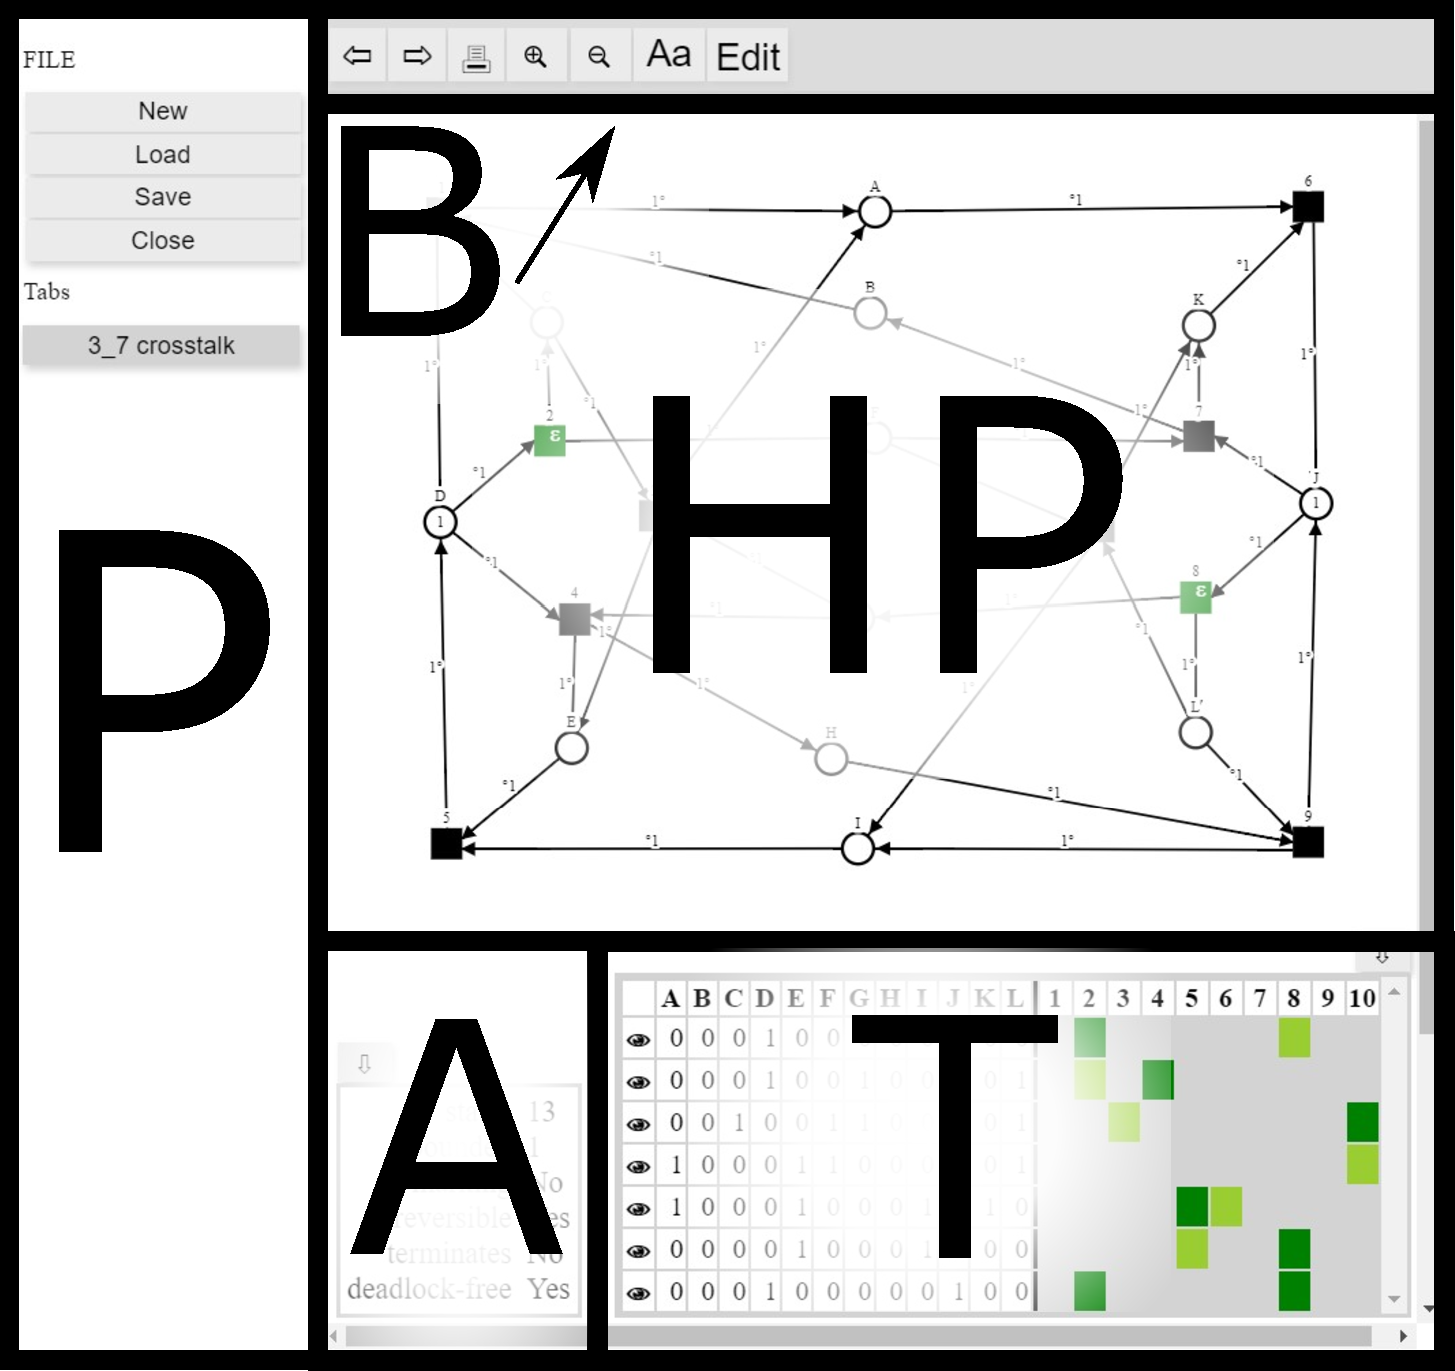
\includegraphics[height=300px, width=350px]{full_image_splited}
  \end{subfigure}
  \caption{Rozložení editoru}
  \label{fig:Rozložení editoru}
  \begin{subfigure}[h]{0.55\textwidth}
    \begin{tabular}{|c l c|}
      \hline
      označení &      název části editoru &    sekce \\
      \hline
      \hline
      P &             Postranní panel&  \ref{panel} \\
      HP &            Hlavní plocha editoru&  \ref{hlavní plocha} \\
      B &             Panel nástrojů editoru &  \ref{panel nástrojů} \\
      T &             Tabulka ohodnocení &  \ref{tabulka ohodnocení} \\
      A &             Výsledky analýzy &  \ref{výsledky analýzy} \\
      \hline
    \end{tabular}
  \end{subfigure}
\end{figure}



\subsubsection{Postranní panel}\label{panel}
\subsubsection{Hlavní plocha editoru}\label{hlavní plocha}
\subsubsection{Panel nástrojů editoru}\label{panel nástrojů}
\subsubsection{Tabulka ohodnocení}\label{tabulka ohodnocení}
\subsubsection{Výsledky analýzy}\label{výsledky analýzy}


\subsubsection{Ovládání}

\subsubsection{Tisk sítě}
\todo{obrázek jak vytisknotu do PDF}

\subsubsection{Klávesové zkratky}





\section{Použité technologie}

\subsection{nodejs}
Aplikace je psaná za pomoci opensourcové technologie nodeJS, která umožňuje využívat jazyk
JavaScript pro psaní serverových aplikací. Cílem platformy nodeJS je vytvořit
ekosystém pro jednoduší vývoj webových stránek a aplikací kde stačí pro vyrvaření
funkcionality pouze jeden programovací jazyk.

\subsection{Typescript}
Typescript je opensource programovací jazyk od společnosti Microsoft který je nadstavbou nad jazykem JavaScript.
Jelikož je Typescript nadstavbou nad programovacím jazykem JavaScript tak je jakýkoliv validní kód v JavaScriptu automaticky validním kódem v Typescriptu.
Typecript se kompiluje do Javascriptu a proto po stránce funkcionality nenabízí nic navíc avšak po stránce vývoje nabízí možnost statické typové kontroly
se kterou je spjaté fungování našeptávačů v dnešních textových editorech a také nabízí možnost kompilace do starších verzí JavaScript se simulací funkcionality novejších verzí JavaScriptu.
\todo{příklady kódu ?}


\subsection{Electron}
Electron je opensource framework pro vytváření desktopových aplikací pomocí webových technologií JavaScript, HTML a CSS.
Využívá NodeJS


\subsection{Javascriptová Knihovna Data driven documents (D3)}
\todo{příklady kódu ?}

\subsection{Scalable Vector Graphics (SVG)}
\todo{příklady kódu ?}




\section{Stavba programu}

\subsection{Třída 1}
\subsection{Třída 2}
\subsection{Třída 3}
\subsection{Třída 4}

























































































\todo{pokračování ukázkového textu}

\noindent\textcolor{red}{\LARGE Upozornění: Následující text
  dokumentace stylu, vyjma přílohy~\ref{sec:ObsahCD}, je rozpracovaná
  a (značně) neúplná verze!!!}

\section{Styly pro psaní bakalářských a diplomových prací}
Toto jsou styly pro psaní bakalářských a diplomových prací přes typografický systém \LaTeX{}, tedy \textbf{kistyles}.

\subsection{Požadavky a podprovaná prostředí}
Sada balíku \textbf{kistyles} podporuje následující distribuce systému \LaTeX{}:
\begin{itemize}
  \item \TeX{} Live.
\end{itemize}

Jsou podporovány všechny výstupní ovladače, tedy jak \textbf{dvi}, tak \textbf{pdf} i \textbf{ps}. Funkčnost zmiňovaných distribucí byla ověřena na několika operačních systémech, mezi které patří:
\begin{enumerate}
  \item Windows $8.1$,
  \item Archlinux,
  \item Debian.
\end{enumerate}

Důrazně se doporučuje používat aktuální verzi dané distribuce systému \LaTeX{}.

%%%  Po přeložení programem CSLaTeX (třikrát) je potřeba použít
%%%  program DVIPS a takto získaný PostScriptový soubor vytisknout
%%%  na PostScriptové tiskárně nebo pomocí programu GhostScript.
%%%
%%%  Rovněž je možné použít program DVIPDFM a vytvořit z dokumentu
%%%  soubor ve formátu PDF včetně hypertextových odkazů.

\subsection{Přepínače}
Styl kidiplom je z hlediska uživatele zastoupen ekvivalentně nazvanou třídou, kterou je třeba volat na záčátku dokumentu:
\begin{kicode}{TeX}{}{Volání třídy \textbf{kidiplom}}
  \documentclass[
    master=true,
    font=sans,
    printversion=false,
    joinlists=true,
    glossaries=true,
    figures=true,
    tables=true,
    sourcecodes=true,
    theorems=true,
    bibencoding=utf8,
    language=czech,
    encoding=utf8,
    field=inf,
    index=true,
    biblatex=true
  ]{kidiplom}
\end{kicode}

Následuje přehled přepínačů, je vždy uvedeno jméno přepínač, včetně výchozí hodnoty. Přepínače uvádí tabulka \ref{tab:prepinace}.

\begin{table}
  \begin{center}
    \caption{Seznam přepínačů}\label{tab:prepinace}
    \scalebox{0.95}{\begin{tabular}{>{\bfseries}l >{\ttfamily}c L{8cm}}
        {\normalfont Přepínač} & {\normalfont Výchozí hodnota} & {\normalfont Popis}                                                                                                  \\
        \hline
        master                 & false                         & Povolí nebo zakáže režim diplomové práce. Výchozí režim je tedy bakalářská práce.                                    \\

        field                  & ainfp                         & Specifikuje studijní obor:\newline
        \begin{description}
          \item[ainf] Aplikovaná informatika\,--\,prezenční,
          \item[ainfk] Aplikovaná informatika\,--\,kombinovaná,
          \item[inf] Informatika\,--\,prezenční,
          \item[infv] Informatika ve vzdělávání\,--\,kombinovaná,
          \item[binf] Bioinformatika\,--\,prezenční.
        \end{description}                                                                                                                                                     \\

        font                   & serif                         & Zapne či vypne podporu pěkného bezpatkového fontu. Možné hodnoty jsou:\newline
        \begin{description}
          \item[sans] Bezpatkové písmo (písmo Iwona).
          \item[serif] Patkové písmo (písmo Computer Modern).
        \end{description}                                                                                                                                                     \\

        %%  'encoding=kódování' pro kódování tohoto a vložených zdrojových
        %%  textů v kódování jiném než výchozím utf8
        encoding               & utf8                          & Kódování souboru dokumentu, doporučuje se ponechat výchozí hodnotu.                                                  \\

        bibencoding            & utf8                          & Kódování souboru bibliografie. Tato volba má smysl pouze, pokud je použita bibliografie skrze balíček \BibLaTeX{}.   \\

        language               & czech                         & Jazyk práce.                                                                                                         \\

        printversion           & false                         & Je-li zapnuto, pak budou odkazy vysázeny optimalizovaně pro knižní sazbu. Tuto volbu je nutno použít pro tisk práce. \\

        %%% Nepovinné argumenty `tables' a `figures' použijte pouze v případě,
        %%% že váš dokument obsahuje tabulky a obrázky a chcete vytvořit
        %%% jejich seznamy za obsahem.
        %%%
        %%% Argument `joinlists' způsobí zřetězení obsahu a seznamů tabulek a obrázků.
        %%% Není-li použít, všechny seznamy jsou uvedeny na samostatných stránkách.

        joinlists              & true                          & Je-li zapnuto, pak seznamy obrázků, tabulek, vět a
        zdrojových kódů sázené za obsahem nebudou rozděleny na samostatné stránky.                                                                                                    \\

        figures                & true                          & Je-li zapnuto, pak v seznamech položek bude zahrnut seznam obrázků.                                                  \\

        tables                 & true                          & Je-li zapnuto, pak v seznamech položek bude zahrnut seznam tabulek.                                                  \\

        theorems               & false                         & Je-li zapnuto, pak v seznamech bude zahrnut seznam teorémů.                                                          \\

        sourcecodes            & false                         & Je-li zapnuto, pak v seznamech bude zahrnut seznam zdrojových kódů.                                                  \\

        glossaries             & false                         & Je-li zapnuto, pak na konci dokumentu bude vysázen seznam zkratek.                                                   \\

        index                  & false                         & Zapíná podporu sazby rejstříku.                                                                                      \\

        biblatex               & true                          & Zapne sazbu bibliografie přes balík \BibLaTeX{}.
      \end{tabular}}
  \end{center}
\end{table}

\subsection{Geometrie stránky}
Tento styl používá list velikosti $A4$. Pro sazbu prací je třeba použít jednostrannou sazbu. Levý okraj je rozšířen s ohledem na vazbu výsledné knižní podoby práce.









\section{Sazba částí dokumentu}
\subsection{Sazba úvodní strany či obsahu}
Vysázení všech podstatných částí úvodu práce obstará makro \kiinlinecode{TeX}{!}{\\maketitle}. Pro správné vysázení všech částí a meta-informací je potřeba použí makra \kiinlinecode{TeX}{!}{\\title}, \kiinlinecode{TeX}{!}{\\author} a další. Jejich přehled lze najít ve zdrojovém souboru tohoto dokumentu. V případě použítí \textbf{pdf} výstupu se generuje i dodatečná hlavička souboru s meta-informacemi jako je autor dokumentu, název práce či dalšími.

\subsection{Závěry}
Závěr práce by se měl poskytnout jak v původním jazyce práce, tak v jazyce anglickém. Pro sazbu závěru jsou k dispozici příslušná makra. Berte na vědomí, že v anglickém závěru se aktivuje plně anglická sazba se všemi konvencemi. Tedy je třeba používat anglické uvozovky a další správné typografické prvky.

\begin{kicode}{TeX}{}{Sazba závěrů}
  % Tiskne český závěr práce.
  \begin{kiconclusions}
    Závěr práce v \uv{českém} jazyce.
  \end{kiconclusions}

  % Tiskne anglický závěr práce.
  \begin{kiconclusions}[english]
    Thesis conclusions written in \uv{English}.
  \end{kiconclusions}
\end{kicode}

\subsection{Matematika}
Pro sazbu matematiky je k dispozici sada standardních maker.
$$\langle f \rangle, \lfloor g \rfloor,
  \lceil h \rceil, \ulcorner i \urcorner$$

$$\left\{\frac{x^2}{y^3}\right\}$$

$$
  A_{m,n} =
  \begin{pmatrix}
    a_{1,1} & a_{1,2} & \cdots & a_{1,n} \\
    a_{2,1} & a_{2,2} & \cdots & a_{2,n} \\
    \vdots  & \vdots  & \ddots & \vdots  \\
    a_{m,1} & a_{m,2} & \cdots & a_{m,n}
  \end{pmatrix}
$$

$$
  M = \begin{bmatrix}
    \frac{5}{6} & \frac{1}{6} & 0           \\[0.3em]
    \frac{5}{6} & 0           & \frac{1}{6} \\[0.3em]
    0           & \frac{5}{6} & \frac{1}{6}
  \end{bmatrix}
$$

\subsection{Sazba literatury}
Pro sazbu literatury má uživatel dvě možnosti. Může použít služeb balíků \BibLaTeX{}, který je pro \textbf{kistyles} zapnutý, či lze použít manuální sazbu bibliografie.
\subsubsection{Sazba bibliografie přes \BibLaTeX{}}
Při použití tohoto balíku se data o použité literatuře ukládají do dedikovaného textového souboru, ukázku najdete i v tomto stylu pod jménem \kiinlinecode{text}{!}{bibliografie.bib}.

Formát daného souboru je nad rámec této dokumentace a je na každém uživateli, aby si jej nastudoval. Bibliografie se tiskne makrem \kiinlinecode{TeX}{!}{\\printbibliography}. Taktéž v preambuli dokumentu je třeba definovat, který soubor data bibliografie obsahuje, tedy například \kiinlinecode{TeX}{!}{\\bibliography\{bibliografie.bib\}}.

Dokument, který využívá \BibLaTeX{} je následně nutné přeložit jak pomocí překladače zvoleného ovladače, tak pomocí aplikace \kiinlinecode{text}{!}{biber}. Více informací poskytne soubor \kiinlinecode{text}{!}{Makefile} z distribuce tohoto stylu.

Výhodou tohoto přístupu je, že bibliografie se vysází automaticky a (obvykle) není třeba manuální úprava formátování.

\subsubsection{Manuální sazba bibliografie}
Manuální sazba obnáší vysázení prostředí \kiinlinecode{text}{!}{thebibliography} ručně. To je nad rámec tohoto dokumentu. Ukázku tohoto přístupu lze samozřejmě nalézt ve zdrojovém souboru tohoto dokumentu nebo také \href{http://www.math.uiuc.edu/~hildebr/tex/bibliographies.html}{zde}.

Pro aktivaci manuální sazby bibliografie je třeba volat třídu \kiinlinecode{text}{!}{kidiplom} s parametrem \kiinlinecode{text}{!}{biblatex=false}. Mějte, prosím, na paměti, že v tomto módu jsou makra \kiinlinecode{text}{!}{\\bibliography} a \kiinlinecode{text}{!}{\\printbibliography} nedostupná.

\subsection{Drobná makra}
Základní styl definuje hned několik maker pro usnadnění práce. Například makro \kiinlinecode{TeX}{!}{\\buno} vysází řetezec \uv{bez újmy na obecnosti}. Je k dispozici i verze s prvním velkým písmenem, \kiinlinecode{TeX}{!}{\\Buno}.

Je rovněž možno přidávat položky do seznamu zkratek. K tomu slouží makro \kiinlinecode{TeX}{!}{\\newacronym}, které lze použít například jednoduše jako \kiinlinecode{TeX}{!}{\\newacronym\{UPOL\}\{UPOL\}\{\\kitextunivcz\}}. Na danou zkratku se pak lze odkazovat jednoduše, \kiinlinecode{TeX}{!}{\\gls\{UPOL\}}.

Sazba uvozovek respektuje nastavení částí dokumentu, a proto se doporučuje používat makro \kiinlinecode{TeX}{!}{\\uv}. V anglické závěru práce toto platí taky, viz tato PDF ukázka.

Styl podporuje sazbu odstavců v tabulkách, více obsahuje tabulka \ref{tab:odstavce}.

\begin{table}
  \begin{center}
    \caption{Seznam přepínačů}\label{tab:odstavce}
    \begin{tabular}{L{4cm}|R{4cm}|L{4cm}}
      \lipsum[23] & \lipsum[22] & \lipsum[21]
    \end{tabular}
  \end{center}
\end{table}

K dispozici jsou také makra pro sazbu \csharp{} (\kiinlinecode{TeX}{!}{\\csharp}) či \cpp{} (\kiinlinecode{TeX}{!}{\\cpp}).

%% v případě tvorby rejstříku přeložit vygenerovaný soubor .idx
%% programem Makeindex a v případě tvorby seznamu zkratek spustit
%% program Makeglossaries s parametrem jméno souboru zdrojového textu
%% bez přípony a následně opět (dvakrát) přeložit zdrojový text
%% programem pdfLaTeX.

\subsection{Sazba rejstříku}
Sazba rejstříku sestává z několika kroků:

\begin{enumerate}
  \item Je třeba přes volbu \kiinlinecode{TeX}{!}{index=true} rejstříkování povolit.
  \item Použítím makra \kiinlinecode{TeX}{!}{\\index} rejstříkovat vybrané pojmy.
  \item Kompilovat s použitím utility \kiinlinecode{TeX}{!}{makeindex}. Pro specifika tohoto kroku si stačí prohlédnout soubor \kiinlinecode{text}{!}{Makefile}.
\end{enumerate}

Makro \kiinlinecode{TeX}{!}{\\index} je redefinováno tak, že sází klikací odkaz na výraz v rejstříku. Je doporučeno jej použít ihned za výrazem\index{výraz}.

\textbf{Omezení redefinovaného makra \kiinlinecode{TeX}{!}{\\index}}: klikací odkaz nefunguje, pokud použijete konstrukci \kiinlinecode{TeX}{!}{\\index\{výraz|makro\}} (resp. \kiinlinecode{TeX}{!}{\\index\{výraz|(makro\}}), např. \kiinlinecode{TeX}{!}{\\index\{výraz|textit\}}.

Rejstřík lze vysázet pomocí makra \kiinlinecode{TeX}{!}{\\printindex}.

\subsection{Sazba zdrojových kódů}
Styl nabízí dva způsoby sazby zdrojových kódů:

\begin{enumerate}
  \item Sazbu řádkových kódů, například \kiinlinecode{CSS}{!}{background-color: white;}. K tomu slouží makro formátu \kiinlinecode{TeX}{!}{\\kiinlinecode\{jazyk\}\{separátor\}\{kód\}}. Za separátor je vhodné volit jakýkoliv znak, který se nevyskytuje v samotném sázeném zdrojovém kódu. Za jazyk je nutno dosadit jeden z těchto: C, TeX, PHP, HTML, Lisp, SQL, TeX, Python, Java, TutorialD, text, csharp, cpp, JavaScript, CSS.

  \item Sazbu zdrojových kódu do separátních prostředí. Takto vytištěný kód se objeví v seznamu zdrojových kódů. Ukázka například zdrojový kód \ref{kod:cpp}. Ukázku sazby naleznete ve zdrojovém kódu tohoto dokumentu.
\end{enumerate}

\newacronym{UPOL}{UPOL}{\kitextunivcz}

\begin{definition}[Název definice]
  Abcd. Abcd. Abcd. Abcd. Abcd. Abcd. Abcd. Abcd. Abcd. Abcd. Abcd. Abcd. Abcd. Abcd. Abcd. Abcd. Abcd. Abcd. Abcd. Abcd. Abcd. Abcd. Abcd. Abcd. Abcd. Abcd. Abcd. Abcd. Abcd. Abcd. \gls{UPOL}
\end{definition}

\begin{proof}[Název důkazu]
  Abcd. Abcd. Abcd. Abcd. Abcd. Abcd. Abcd. Abcd. Abcd. Abcd. Abcd. Abcd. Abcd. Abcd. Abcd. Abcd. Abcd. Abcd. Abcd. Abcd. Abcd. Abcd. Abcd. Abcd. Abcd. Abcd. Abcd. Abcd. Abcd. Abcd.
\end{proof}

\begin{remark}[Pumpovací věta]
  Abcd. Abcd. Abcd. Abcd. Abcd. Abcd. Abcd. Abcd. Abcd. Abcd. Abcd. Abcd. Abcd. Abcd. Abcd. Abcd. Abcd. Abcd. Abcd. Abcd. Abcd. Abcd. Abcd. Abcd. Abcd. Abcd. Abcd. Abcd. Abcd. Abcd.
\end{remark}

\begin{example}[Pumpovací věta]
  Abcd. Abcd. Abcd. Abcd. Abcd. Abcd. Abcd. Abcd. Abcd. Abcd. Abcd. Abcd. Abcd. Abcd. Abcd. Abcd. Abcd. Abcd. Abcd. Abcd. Abcd. Abcd. Abcd. Abcd. Abcd. Abcd. Abcd. Abcd. Abcd. Abcd.
\end{example}

\begin{lemma}[Název definice]
  Abcd. Abcd. Abcd. Abcd. Abcd. Abcd. Abcd. Abcd. Abcd. Abcd. Abcd. Abcd. Abcd. Abcd. Abcd. Abcd. Abcd. Abcd. Abcd. Abcd. Abcd. Abcd. Abcd. Abcd. Abcd. Abcd. Abcd. Abcd. Abcd. Abcd.
\end{lemma}

\begin{consequence}[Název důkazu]
  Abcd. Abcd. Abcd. Abcd. Abcd. Abcd. Abcd. Abcd. Abcd. Abcd. Abcd. Abcd. Abcd. Abcd. Abcd. Abcd. Abcd. Abcd. Abcd. Abcd. Abcd. Abcd. Abcd. Abcd. Abcd. Abcd. Abcd. Abcd. Abcd.
\end{consequence}

\begin{theorem}[Pumpovací věta]
  Abcd. Abcd. Abcd. Abcd. Abcd. Abcd. Abcd. Abcd. Abcd. Abcd. Abcd. Abcd. Abcd. Abcd. Abcd. Abcd. Abcd. Abcd. Abcd. Abcd. Abcd. Abcd. Abcd. Abcd. Abcd. Abcd. Abcd. Abcd. Abcd. Abcd.
\end{theorem}


\begin{kicode}{cpp}{kod:cpp}{\cpp}
  int main("cs acsa") // komentar
  int main("cs acsa") // komentar
  int main("cs acsa") // komentar
  int main("cs acsa") // komentar
  int main("cs acsa") // komentar
\end{kicode}

\begin{kicode}{JavaScript}{}{JS}
  new object() // komentar
\end{kicode}

\begin{kicode}{csharp}{}{\csharp}
  public static int main("cs acsa") // komentar
\end{kicode}

\begin{kicode}{SQL}{}{SQL}
  SELECT * FROM table_1; /* komentar */
\end{kicode}

\begin{kicode}{TutorialD}{}{TutorialD}
  table_1 AND table_2;
\end{kicode}

%% Závěry práce. V jazyce práce a anglicky. Text pro jiný než
%% nastavený jazyk práce (nepovinným parametrem language makra
%% \documentclass, výchozí český) se zadává použitím makra s uvedením
%% jazyka jako nepovinného parametru.
\begin{kiconclusions}
  Závěr práce v \uv{českém} jazyce.
\end{kiconclusions}

\begin{kiconclusions}[english]
  Thesis conclusions in \uv{English}.
\end{kiconclusions}

%% Přílohy obsahu textu práce, za makrem \appendix.
\appendix

\section{První příloha}
Text první přílohy

\section{Druhá příloha}
Text druhé přílohy

%% Obsah přiloženého CD/DVD. Poslední příloha. Upravte podle vlastní
%% práce!
\section{Obsah přiloženého CD/DVD} \label{sec:ObsahCD}

Na samotném konci textu práce je uveden stručný popis obsahu
přiloženého CD/DVD, tj.~jeho závazné adresářové struktury, důležitých
souborů apod.

\begin{description}

  \item[\texttt{bin/}] \hfill \\
        Instalátor \textsc{Instalator} programu, popř.~program
        \textsc{Program}, spustitelné přímo z~CD/DVD. / Kompletní adresářová
        struktura webové aplikace \textsc{Webovka} (v~ZIP archivu) pro
        zkopírování na webový server. Adresář obsahuje i~všechny runtime
        knihovny a~další soubory potřebné pro bezproblémový běh instalátoru
        a~programu z~CD/DVD / pro bezproblémový provoz webové aplikace na
        webovém serveru.

  \item[\texttt{doc/}] \hfill \\
        Text práce ve formátu PDF, vytvořený s~použitím závazného stylu KI
        PřF UP v~Olomouci pro závěrečné práce, včetně všech příloh,
        a~všechny soubory potřebné pro bezproblémové vygenerování PDF
        dokumentu textu (v~ZIP archivu), tj.~zdrojový text textu, vložené
        obrázky, apod.

  \item[\texttt{src/}] \hfill \\
        Kompletní zdrojové texty programu \textsc{Program} / webové aplikace
        \textsc{Webovka} se všemi potřebnými (příp.~převzatými) zdrojovými
        texty, knihovnami a~dalšími soubory potřebnými pro bezproblémové
        vytvoření spustitelných verzí programu / adresářové struktury pro
        zkopírování na webový server.

  \item[\texttt{readme.txt}] \hfill \\
        Instrukce pro instalaci a~spuštění programu \textsc{Program}, včetně
        všech požadavků pro jeho bezproblémový provoz. / Instrukce pro
        nasazení webové aplikace \textsc{Webovka} na webový server, včetně
        všech požadavků pro její bezproblémový provoz, a~webová adresa, na
        které je aplikace nasazena pro účel testování při tvorbě posudků
        práce a~pro účel obhajoby práce.

\end{description}

Navíc CD/DVD obsahuje:

\begin{description}

  \item[\texttt{data/}] \hfill \\
        Ukázková a~testovací data použitá v~práci a~pro potřeby testování
        práce při tvorbě posudků a~obhajoby práce.

  \item[\texttt{install/}] \hfill \\
        Instalátory aplikací, runtime knihoven a~jiných souborů potřebných
        pro provoz programu \textsc{Program} / webové aplikace
        \textsc{Webovka}, které nejsou standardní součástí operačního
        systému určeného pro běh programu / provoz webové aplikace.

  \item[\texttt{literature/}] \hfill \\
        Vybrané položky bibliografie, příp.~jiná užitečná literatura
        vztahující se k~práci.

\end{description}

U~veškerých cizích převzatých materiálů obsažených na CD/DVD jejich
zahrnutí dovolují podmínky pro jejich šíření nebo přiložený souhlas
držitele copyrightu. Pro všechny použité (a~citované) materiály,
u~kterých toto není splněno a~nejsou tak obsaženy na CD/DVD, je uveden
jejich zdroj (např.~webová adresa) v~bibliografii nebo textu práce
nebo v souboru \texttt{readme.txt}.

%% -------------------------------------------------------------------

%% Sazba volitelného seznamu zkratek, za přílohami.
\printglossary

%% Sazba povinné bibliografie, za přílohami (případně i za seznamem
%% zkratek). Při použití BibLaTeXu použijte makro
%% \printbibliography. jinak prostředí thebibliography. Ne obojí!

%% Sazba i v textu necitovaných zdrojů, při použití
%% BibLaTeXu. Volitelné.
\nocite{*}
%% Vlastní sazba bibliografie při použití BibLaTeXu.
\printbibliography

%% Bibliografie, včetně sazby, při nepoužití BibLaTeXu.
% \begin{thebibliography}{9}
%\bibitem{kniha2} \uppercase{Hawke}, Paul. NanoHttpd: Light-weight HTTP server designed for embedding in other applications. GitHub [online]. 2014-05-12. [cit. 2014-12-06]. Dostupné z: \url{https://github.com/NanoHttpd/nanohttpd}
%
%\bibitem{jeske13} \uppercase{Jeske}, David; \uppercase{Novák}, Josef. Simple HTTP Server in \csharp: Threaded synchronous HTTP Server abstract class, to respond to HTTP requests. CodeProject: For those who code [online]. 2014-05-24. [cit. 2014-12-06]. Dostupné z: \url{http://www.codeproject.com/Articles/137979/Simple-HTTP-Server-in-C}
%
%\bibitem{uzis2012} \uppercase{ÚSTAV ZDRAVOTNICKÝCH INFORMACÍ A STATISTIKY ČR}. Lékaři, zubní lékaři a farmaceuti 2012 [online]. Praha 2, Palackého náměstí 4: Ústav zdravotnických informací a statistiky ČR, 2012 [cit. 2014-12-06]. ISBN 978-80-7472-089-5. Dostupné z: \url{http://www.uzis.cz/publikace/lekari-zubni-lekari-farmaceuti-2012}
% \end{thebibliography}

%% Sazba volitelného rejstříku, za bibliografií.
\printindex

\end{document}
